% !TeX root = main.tex
\chapter{Evaluation Datasets}
\label{appendix:evaluation_tasks}

This appendix summarises the datasets and task models used in Chapter~\ref{chap:evaluation}. The purpose is to make the experimental workload clear without moving task-specific detail into the main systems and method narrative.

\section{Overview}

The evaluation uses three tasks. California Housing provides a lightweight tabular regression control, Fashion-MNIST provides a small image-classification workload, and CIFAR-10 provides the main compute-bound image-classification workload. All three are instantiated through the shared research-app task interface described in Chapter~\ref{chap:implementation}; the run configs then choose the partitioner, method, model-rate assignment, training budget, and deployment.

\section{California Housing Regression}
\label{appendix:california_housing_task}

\paragraph{Dataset.}
California Housing is a tabular regression dataset derived from California census block-group records \parencite{pace1997sparse}. Each example contains eight continuous attributes describing location, occupancy, rooms, population, and income. The prediction target is median house value. The dissertation uses the TensorFlow/Keras cached array with \(20{,}640\) examples, split into \(80\%\) training and \(20\%\) test data with a fixed seed. Features and targets are standardised using training-set statistics before model training.

\begin{figure}[H]
\centering
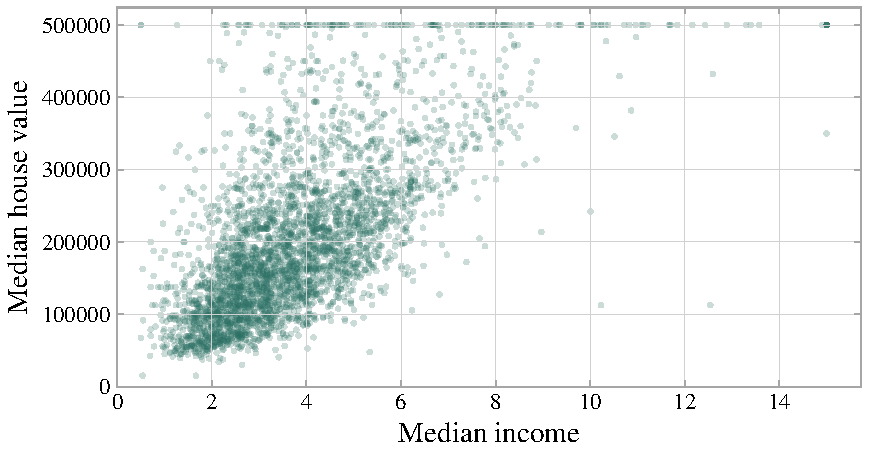
\includegraphics[width=0.56\textwidth]{figures/evaluation_task_california_housing_scatter.pdf}
\caption{\textbf{California Housing target relationship.} The scatter shows a deterministic sample of examples by median income and median house value before standardisation.}
\label{fig:appendix_california_housing_scatter}
\end{figure}

\paragraph{Model and partitioning.}
The task uses a width-scaled MLP with two hidden layers. At full rate, the hidden widths are \(128\) and \(64\); lower model rates reduce those widths while preserving the same input and output structure. IID runs split examples uniformly across clients. Non-IID runs use the continuous partitioner over a configured continuous feature, producing ordered partitions rather than label-skewed classification partitions.

\section{Fashion-MNIST Classification}
\label{appendix:fashion_mnist_task}

\paragraph{Dataset.}
Fashion-MNIST is a \(10\)-class image-classification dataset of clothing and accessory images \parencite{xiao2017fashionmnist}. Each example is a \(28\times28\) greyscale image. The dataset contains \(60{,}000\) training examples and \(10{,}000\) test examples. The implementation converts images to tensors and normalises them with mean \(0.2860\) and standard deviation \(0.3530\).

\begin{figure}[H]
\centering
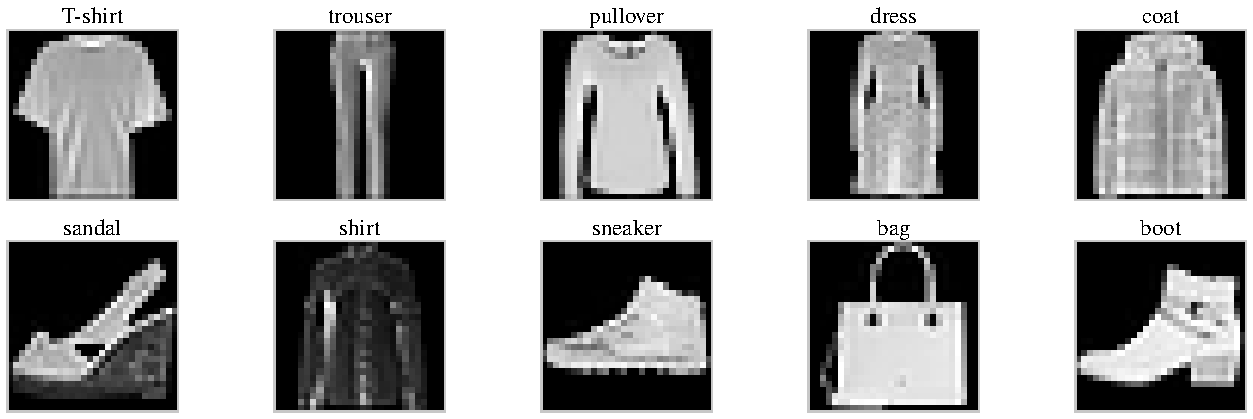
\includegraphics[width=0.64\textwidth]{figures/evaluation_task_fashion_mnist_samples.pdf}
\caption{\textbf{Sample Fashion-MNIST images.} One example is shown for each class.}
\label{fig:appendix_fashion_mnist_samples}
\end{figure}

\paragraph{Model and partitioning.}
The task uses a compact width-scaled CNN with two convolutional blocks and a linear classifier. At full rate, the convolutional widths are \(32\) and \(64\); lower model rates reduce the channel counts. IID runs split examples uniformly across clients. Non-IID runs use Dirichlet label-skew partitioning with \(\alpha=0.3\), matching the CIFAR-10 image-classification regime used for the main method comparisons.

\section{CIFAR-10 Classification}
\label{appendix:cifar10_task}

\paragraph{Dataset.}
CIFAR-10 is a standard \(10\)-class natural-image classification dataset \parencite{krizhevsky2009cifar}. Each example is a \(32\times32\) RGB image, and the dataset contains \(50{,}000\) training examples and \(10{,}000\) test examples. The implementation converts images to tensors and normalises channels with mean \((0.4914,0.4822,0.4465)\) and standard deviation \((0.2470,0.2435,0.2616)\).

\begin{figure}[H]
\centering
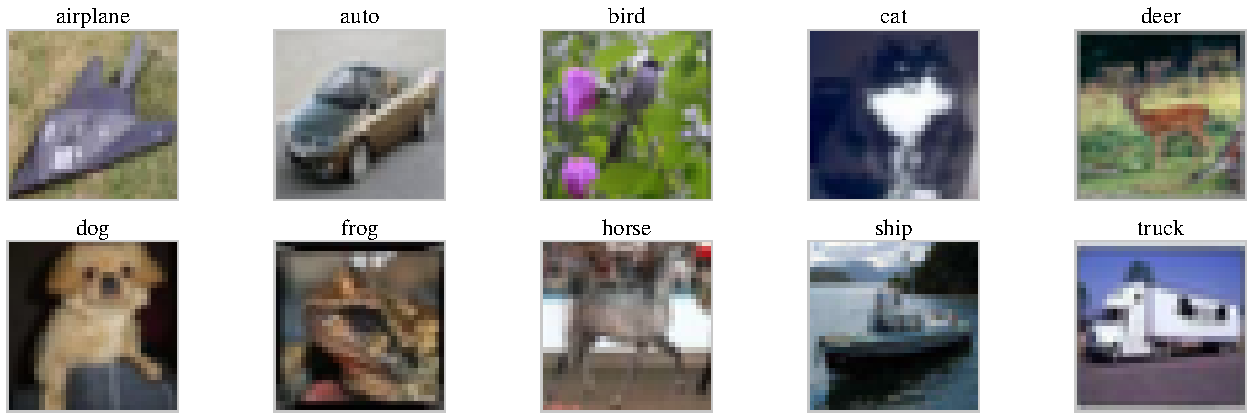
\includegraphics[width=0.64\textwidth]{figures/evaluation_task_cifar10_samples.pdf}
\caption{\textbf{Sample CIFAR-10 images.} One example is shown for each class.}
\label{fig:appendix_cifar10_samples}
\end{figure}

\paragraph{Model and partitioning.}
The task uses a width-scaled CNN with three convolutional blocks, adaptive average pooling, and a linear classifier. At full rate, the convolutional widths are \(64\), \(128\), and \(256\). This makes CIFAR-10 the most compute-bound workload in the evaluation and the clearest test of whether submodel FL reduces local training cost. IID runs split examples uniformly across clients, while non-IID runs use Dirichlet label-skew partitioning with \(\alpha=0.3\).
